\begin{titlingpage}

\newcommand\nbvspace[1][3]{\vspace*{\stretch{#1}}}
% allow some slack to avoid under/overfull boxes
\newcommand\nbstretchyspace{\spaceskip0.5em plus 0.25em minus 0.25em}
% To improve spacing on titlepages
\newcommand{\nbtitlestretch}{\spaceskip0.6em}
\pagestyle{empty}

\begin{center}
\bfseries
\nbvspace[1]

\Large Ajay Agrawal, Joshua Gans, Avi Golddfarb\\
\Huge
{\nbtitlestretch\Huge La economía de la inteligencia artificial: una agenda}\\
\vspace{.5cm}
\large

\nbvspace[1]

APUNTES\\

\nbvspace[1]
\small POR\\
\Large FODE\\[0.5em]
\footnotesize CHRISTIAN LIMBERT PAREDES AGUILERA\\

\nbvspace[2]

\begin{center}
    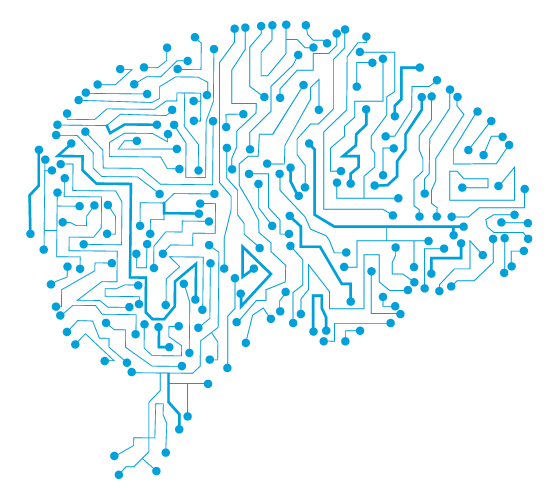
\includegraphics[width=0.5\textwidth]{img/ia.png}
\end{center}

\nbvspace[3]
\normalsize

\nbvspace[1]

\end{center}

\break
\bfseries 

\nbvspace[1]
The University of Chicago Press, Chicago 60637\\
The University of Chicago Press, Ltd., London\\
 2019 by the National Bureau of Economic Research, Inc.\\
All rights reserved. No part of this book may be used or reproduced\\
in any manner whatsoever without written permission, except in the\\
case of brief quotations in critical articles and reviews. For more\\
information, contact the University of Chicago Press, 1427 E. 60th St.,\\
Chicago, IL 60637.\\
Published 2019\\
Printed in the United States of America\\
\nbvspace[1]

\begin{center}
Sin ninguna revisión de esta obra.\\


\nbvspace[1]
    Propiedad de esta obra:\\ 

    CHRISTIAN LIMBERT PAREDES AGUILERA\\	

    E-mail: soyfode@gmail.com
\end{center}

\nbvspace[1]

Reservados todos los derechos. La reproducción total o parcial de esta obra, por cualquier medio o procedimiento, comprendidos la reprografía y el tratamiento informático, y la distribución de ejemplares de ella mediante alquiler o préstamo públicos, queda rigurosamente prohibida sin la autorización escrita de los titulares del copyright, bajo las sanciones establecidas por las leyes.\\

\center 2022 

\end{titlingpage}


\pagenumbering{roman}

\tableofcontents								%indice

\pagestyle{fancy}
\fancyhead[LE,RO]{\nouppercase{\truncate{0.5\headwidth}{\rightmark}}}
\fancyhead[LO,RE]{\nouppercase{\truncate{0.5\headwidth}{\leftmark}}}


